\documentclass[a4paper,11pt]{article}
\usepackage[T1]{fontenc}
\usepackage[utf8]{inputenc}
\usepackage{lmodern}
\usepackage{amsmath}
\usepackage{amsfonts}
\usepackage{amssymb}
\usepackage{amsthm}
\usepackage{graphicx}
\usepackage{color}
\usepackage{xcolor}
\usepackage{url}
\usepackage{textcomp}
\usepackage{parskip}
\usepackage{tikz} 

\title{Solving Alphametics}
\author{Sven Bijleveld}
\date{\today}

\begin{document}

\maketitle
\tableofcontents

\pagebreak

\section{Problem Definition}
We want to find a set of operations to solve an alphametic puzzle. An example of such a puzzle is this:

\begin{center}
\begin{tabular}{ c c c c c c } 
   &   & S & E & N & D \\ 
 + &   & M & O & R & E \\
 \hline 
 = & M & O & N & E & Y \\ 
 
\end{tabular}
\end{center}

Where

\begin{itemize}

\item $ E, N, O, R, Y \in \mathbb{N}_0 $ and $ M, S \in \mathbb{N}$

\item $ E \neq N \neq O \neq R \neq Y \neq M \neq S \neq E $

\item{
\begin{align*}
  Y &= D + E &\left(\mod 10\right) \\
  E &= N + R + \lfloor\frac{D + E}{10}\rfloor &\left(\mod 10\right) \\
  N &= E + O + \lfloor\frac{N + R + \lfloor\frac{D + E}{10}\rfloor}{10}\rfloor &\left(\mod 10\right) \\
    & \vdots \nonumber
\end{align*}
}
\end{itemize}

We can introduce a term $c_n$ for the overflow where $c \in \{0, 1\} $ in this case. 

\begin{flalign*}
    Y &= D + E       &\left(\mod 10\right) \\
    E &= N + R + c_1 &\left(\mod 10\right) \\
    N &= E + O + c_2 &\left(\mod 10\right) \\
    O &= S + M + c_3 &\left(\mod 10\right) \\
    M &=         c_4 &\left(\mod 10\right) 
\end{flalign*}

$c_{max}$ can be generalized as it is linked to the number of addends where $c_{max} = \max\{n_{addends} - 1, 9\} $

\pagebreak
\section{A Simpler Example}
Let's experiment by solving a simple example 


\begin{center}
\begin{tabular}{ c c c c} 
   &   & T & O \\ 
 + &   & G & O \\
 \hline 
 = & O & U & T \\ 
 
\end{tabular}
\end{center}

This alphametic results in the following equations

\begin{align}
    T &= O + O       &(\mod 10) \label{eg:eq1} \\
    U &= T + G + c_1 &(\mod 10) \label{eq:eq2} \\
    O &=         c_2 &(\mod 10) \label{eq:eq3}
\end{align}

We can construct a graph like structure to see what variables depend on each other:

\begin{center}
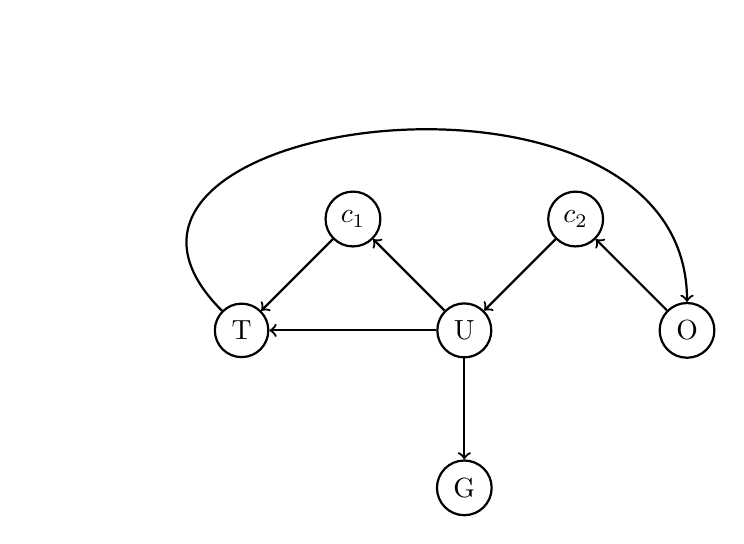
\begin{tikzpicture}[node distance={20mm}, thick, main/.style = {draw, circle}] 
    \node[main] (1)                    {T};
    \node[main] (5) [above right of=1] {$c_1$};
    \node[main] (2) [below right of=5] {U};
    \node[main] (6) [above right of=2] {$c_2$};
    \node[main] (3) [below right of=6] {O}; 
    \node[main] (4) [below       of=2] {G};
    \draw[->] (1) to [out=135,in=90,looseness=1.5] (3);
    \draw[->] (2) -- (1);
    \draw[->] (2) -- (4);
    \draw[->] (2) -- (5);
    \draw[->] (3) -- (6);
    \draw[->] (5) -- (1);
    \draw[->] (6) -- (2);
\end{tikzpicture} 
\end{center}

\pagebreak
\section{Solving the more complicated case}

the alphametic from the introduction above gives us the following graph

\begin{center}
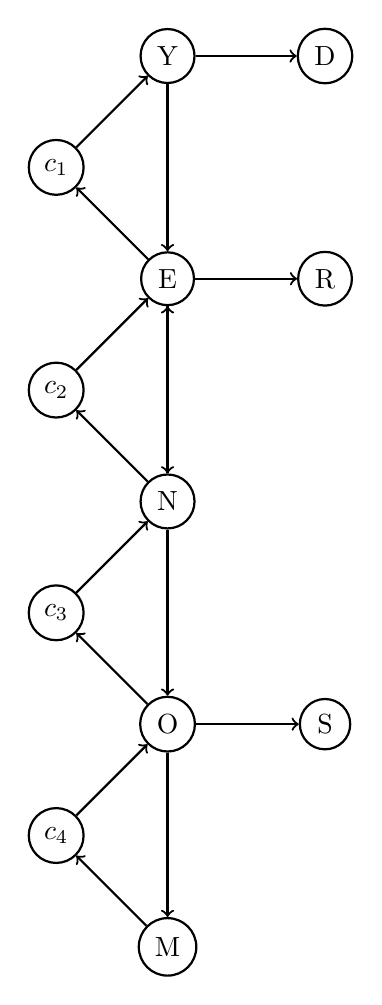
\begin{tikzpicture}[node distance={20mm}, thick, main/.style = {draw, circle}] 
    \node[main] (1)                       {Y};
    \node[main] (9)  [below left    of=1] {$c_1$};
    \node[main] (2)  [below right   of=9] {E}; 
    \node[main] (10) [below left    of=2] {$c_2$};
    \node[main] (3)  [below right  of=10] {N};    
    \node[main] (11) [below left    of=3] {$c_3$};
    \node[main] (4)  [below right  of=11] {O};
    \node[main] (12) [below left    of=4] {$c_4$};
    \node[main] (5)  [below right  of=12] {M};
    \node[main] (6)  [right         of=1] {D};
    \node[main] (7)  [right         of=2] {R};
    \node[main] (8)  [right         of=4] {S};
    
    
    
    \draw[->] (1) -- (2);
    \draw[->] (1) -- (6);
    
    \draw[->] (2) -- (3);
    \draw[->] (2) -- (7);
    \draw[->] (2) -- (9);
    
    \draw[->] (3) -- (2);
    \draw[->] (3) -- (4);
    \draw[->] (3) -- (10);
    
    
    \draw[->] (4) -- (5);
    \draw[->] (4) -- (8);
    \draw[->] (4) -- (11);
    
    \draw[->] (5) -- (12);
    
    \draw[->] (9) -- (1);
    \draw[->] (10) -- (2);
    \draw[->] (11) -- (3);
    \draw[->] (12) -- (4);
    
\end{tikzpicture} 
\end{center}

\end{document}